% !TEX root = ./multilinear.tex
\section{Preliminaries}
\label{sec:prelim}

\subsection{The Multilinear Detection Problem}
Let $X = x_1, \ldots,x_n$ be a set of variables, and let $P(X)$ be a polynomial, which is a sum 
of monomials on $X$. We will denote $P(X)=\sum_S \Pi_{i\in S} x_i$ as a monomial, where
the sum is over multisets $S$.  An example of a polynomial on six variables is 
$P(x_1,x_2,x_3,x_4, x_5, x_6) = x_1^2x_2 + x_2x_3x_4 + x_3x_4x_5 + x_5x_6$. 
A monomial is called \emph{multilinear} or \emph{square-free} if all its variables 
have exponent 1, and its \emph{degree} is the sum of the exponents of all its variables. 
For instance, in the example above, $x_2x_3x_4$, $x_3x_4x_5$, and $x_5x_6$ are multilinear monomials, but $x_1^2x_2$ is not multilinear. 
Given variables $X = x_1, \ldots ,x_n$ and a polynomial $P(X)$, the goal in 
the $k$-Multilinear Detection (\textsc{$k$-MLD}) problem
is to decide whether or not $P(X)$ has a multilinear monomial of degree exactly $k$. 


We note that the polynomial $P(X)$ may have an arbitrary number of terms---i.e., exponential on the size of $n$---therefore, the problem is not as simple as writing the polynomial explicitely and checking each term. Rather, we assume that $P(X)$ is given succintly in a recursive form, and the ``yes"/``no" decision has to be made without unrolling this recursion.
Figure \ref{fig:dag} illustrates a circuit representation of the polynomial $P(\cdot)$ above.
In general, we also have a weight $w_S$ for each multinomial $\Pi_{i\in S} x_i$ corresponding
to each term in the polynomial $P(\cdot)$. Our focus in this paper will be the following problem.

\begin{figure}[h]
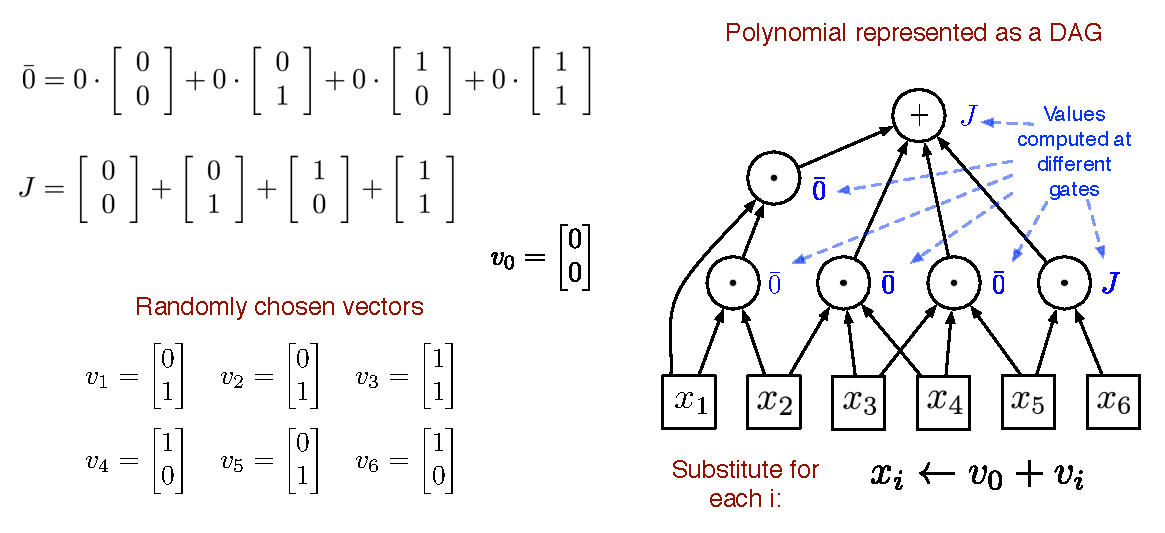
\includegraphics[width=0.5\textwidth]{img/dag3_fixed.pdf}
\caption{
\small
The polynomial $P(x_1,x_2,x_3,x_4, x_5, x_6) = x_1^2x_2 + x_2x_3x_4 + x_3x_4x_5 + x_5x_6$
represented as a circuit with multiplication ($\cdot$) and addition ($+$) gates, which is a DAG. 
Each variable $x_i$ is assigned the element $v_0+v_i\in\mathbb{Z}_2[\mathbb{Z}_2^2]$,
for randomly chosen $v_i\in \mathbb{Z}_2^2$. The computations at each gate
are in the group algebra, and are shown in blue. The circuit evaluates to the element $J$.
\vspace{-0.2in}
}
\label{fig:dag}
\end{figure}

\begin{problem} (\textsc{$k$-MLD} problem)
Given a polynomial $P(\cdot)$ represented by a DAG $G=(V, E)$, in which each monomial
has degree at most $k$, with a weight $w_S$ for
each monomial corresponding to the multiset $S$ in $P(\cdot)$, determine:
(1) if $P(\cdot)$ has a multilinear term, and 
(2) the maximum weight of any multilinear term, if one exists.
\end{problem}


\subsection{Group Algebras}
\label{sec:grpalgebra}
We discuss some notation from group algebras that is crucial for the paper. 
Let $\mathbb{Z}_2^k$ be the group formed by all the $k$-dimensional binary vectors, and define the group multiplication operation as entry-wise XOR. For example, $\mathbb{Z}_2^2$ consists of the vectors $v_0 = (0, 0), v_1 = (0, 1), v_2 = (1, 0), v_3 = (1, 1)$. We note that $v_0$ is the multiplicative identity of the group, and each element is its own multiplicative inverse: $v_i \cdot v_i = v_0$. Now, we define a group algebra $\mathbb{Z}_2[\mathbb{Z}_2^k]$. Each element in the group algebra is a sum of elements from $\mathbb{Z}_2^k$ with coefficients from $\mathbb{Z}_2$ (i.e., either 1 or 0):
$
\sum_{v\in \mathbb{Z}_2^k} a_v v,
$
where $a_v \in \{0,1\}$. The addition operator of the group algebra is
{\scriptsize
$$
\sum_{v\in \mathbb{Z}_2^k} a_v v + \sum_{v\in \mathbb{Z}_2^k} b_v v = \sum_{v\in \mathbb{Z}_2^k} (a_v + b_v) v,
$$}
where the addition of the coefficients is modulo 2, and the multiplication is defined as
{\scriptsize
$$
\left(\sum_{v\in \mathbb{Z}_2^k} a_v v\right)\left(\sum_{u\in \mathbb{Z}_2^k} b_u u\right) = \sum_{v\in \mathbb{Z}_2^k} (a_v \cdot b_u) (v\cdot u).
$$}


\begin{mdframed}
\scriptsize{
\noindent
\textbf{Example.} For $k=2$, the group algebra $\mathbb{Z}_2[\mathbb{Z}_2^k]$ has
$2^{2^2}=16$ elements, such as
\[
x_1=
0\cdot
\begin{bmatrix}
0\\
0
\end{bmatrix}
+ 1\cdot
\begin{bmatrix}
0\\
1
\end{bmatrix}
+
1\cdot
\begin{bmatrix}
1\\
0
\end{bmatrix}
+ 0\cdot
\begin{bmatrix}
1\\
1
\end{bmatrix}
, \mbox{ which we also write as }
\begin{bmatrix}
0\\
1
\end{bmatrix}
+
\begin{bmatrix}
1\\
0
\end{bmatrix}
\]


\[
x_2 =
\begin{bmatrix}
0\\
0
\end{bmatrix}
+
\begin{bmatrix}
1\\
0
\end{bmatrix}
\]

We have 
\[
x_1 + x_2 = 
\begin{bmatrix}
0\\
0
\end{bmatrix}
+
\begin{bmatrix}
0\\
1
\end{bmatrix}
+ 2
\begin{bmatrix}
1\\
0
\end{bmatrix}
=
\begin{bmatrix}
0\\
0
\end{bmatrix}
+
\begin{bmatrix}
0\\
1
\end{bmatrix}
\]

\[
x_1x_2 = 
\left(
\begin{bmatrix}
0\\
1
\end{bmatrix}
+ 
\begin{bmatrix}
1\\
0
\end{bmatrix}
\right)\cdot 
\left(
\begin{bmatrix}
0\\
0
\end{bmatrix}
+
\begin{bmatrix}
1\\
0
\end{bmatrix}
\right) =
\begin{bmatrix}
0\\
0
\end{bmatrix}
+
\begin{bmatrix}
0\\
1
\end{bmatrix}
+
\begin{bmatrix}
1\\
0
\end{bmatrix}
+
\begin{bmatrix}
1\\
1
\end{bmatrix}
\]
It is easy to check that
\[
x_1^2x_2 = 
0\cdot
\begin{bmatrix}
0\\
0
\end{bmatrix}
+ 0\cdot
\begin{bmatrix}
0\\
1
\end{bmatrix}
+ 0\cdot
\begin{bmatrix}
1\\
0
\end{bmatrix}
+ 0\cdot
\begin{bmatrix}
1\\
1
\end{bmatrix}
= \mathbf{\bar{0}} \text{ (additive identify)}
\]
}
\end{mdframed}

\subsection{Applications of parallel multilinear detection}
\label{sec:applications}
Multilinear detection has a broad class of applications\cite{DBLP:journals/talg/KoutisW16,cadena:sdm17}, two of which we summarize below. The first involves finding paths and trees in a graph---Koutis et al.
\cite{DBLP:journals/talg/KoutisW16} showed that these problems can be solved using multilinear detection. The second problem involves anomaly detection using the approach known as graph scan statistics. This was solved sequentially using
the color coding technique in \cite{cadena:sdm17}.
%As before, $G = (V, E)$, denotes a graph where $V$ is a set of $n$ vertices or nodes, and $E$ is a set of $m$ edges. Let $\nbr{v}=\{u: (u,v)\in E\}$ denote the set of neighbors of node $v$.

\subsubsection{Finding Paths and Trees}
\label{sec:apps-trees}
Given a graph $G=(V, E)$ with $n=|V|$, $m=|E|$, and a subgraph $H=(V_H, E_H)$, with $k=|V_H|$, the basic subgraph isomorphism problem involves finding a mapping $f:V_H\rightarrow V$
such that $(i, j)\in E_H$ if and only if $(f(i), f(j))\in E$.

\begin{problem} ($k$-Tree)
\label{prob:trees}
Given a weighted graph $G=(V, E)$ with a weight vector $\mathbf{w}$, and a tree
denoted by $H=(V^H, E^H)$ with $|V^H|=k$, the objective is to determine if there exists
an embedding of $H$ in $G$.
\end{problem}

We show below that Problem \ref{prob:trees} can be solved by formalizing it as a multilinear detection problem. We first consider the case where $H$ is a path of length $k$, for notational simplicity. Let $x_v$ denote a variable associated with each node $v\in V$. We define poynomials $P_v(i)$ for all $v\in V$, $i\leq k$ in the following manner.
\begin{itemize}
\item
$P_v(1) = x_v$ for all $v\in V$
\item
For $i>1$,
$P_v(i) = \sum_{i'<i} \sum_{u\in\nbr(v)} P_u(i')P_v(i-i')$
\item
Define the polynomial $P(x_1,\ldots,x_n) = \sum_v P_v(k)$
\end{itemize}
It can be verified that the graph $G$ has a path of length $k$ if and only if the polynomial $P(x_1,\ldots,x_n)$ has a multilinear term.

\subsubsection{Anomaly Detection Using Graph Scan Statistics}
\label{sec:apps-scanstat}
We use the notation of \cite{cadena:sdm17} here. We assume each node $v\in V$ has two associated values,
which vary with time (we will not show the time, to avoid complicating the notation):
(1) a \emph{baseline count}, $b(v)$, which indicates the count that we
expect to see at the node $v$---e.g., the number of people in a county corresponding to node $v$---and
(2) an \emph{event count} or \emph{weight}, $w(v)$, which indicates how many occurrences of an event
of interest are seen at the node---e.g., the number of cases of a disease in a county.

Graph scan statistics are among the most commonly used methods for detecting anomalies or ``hotspots" in
networked data \cite{Speakman-14,leiserson2015pan, hansen2016finding, neil2013scan, chen2014non}.
Informally, this approach formalizes anomaly detection as a hypothesis testing problem.
Under the null hypothesis $H_0$, it is \emph{business as usual}, and the event counts for all nodes are generated proportionally to their baseline counts. Under the alternative hypothesis $H_1(S)$, counts of a majority of
the vertices are generated (again) with rate proportional to the baseline counts, but there exists a small connected subset
$S \subseteq V$ of vertices for which the counts are generated at a higher rate than expected.
Then, the goal is to find a set of vertices $S$ that maximizes an appropriate scan statistic function $F(S)$, typically a log-likelihood ratio that compares event counts to baseline counts. We define a scan statistic in terms of the event and baseline counts of a node set:
$$
F(S) = F(W(S), B(S), \mathbf{\theta}),
$$
where $W(S) = \sum_{v \in S} w(v)$ is the total event count or \emph{weight} of $S$, $B(S) = \sum_{v \in S} b(v)$ is the baseline count of the set, and $\theta$ represents possible additional arguments to $F$.

%Depending on the assumptions that are satisfied by the data, there are two broad types of scan statistics: parametric and non-parametric.
%An example of a non-parametric function is the Berk-Jones scan statistic (BJ) \cite{Berk-79} used for civil unrest events and network intrusion detection~\cite{chen2014non,mcfowland2013fast}. In this setting, each node $v$ has a $p$-value $p(v) \in [0,1]$, and, for a significance level $\alpha$, the event count $w(v)$ is 1 if $p(v) < \alpha$ (i.e., the node is significant) and 0 otherwise, and the baseline count is $b(v) = 1$ for all nodes. This scan statistic is defined as
%{\scriptsize
%$$
%\max_{\alpha \leq \alpha_{max}}B(S) \left[\frac{W(S)}{B(S)} \log\left(\frac{\frac{W(S)}{B(S)}}{\alpha}\right) + \left(1 - \frac{W(S)}{B(S)}\right) \log\left(\frac{1 - \frac{W(S)}{B(S)}}{1 -\alpha}\right) \right],
%$$}
%with $\mathbf{\theta} = \alpha_{max}$.
%A well-known example of a parametric function is the Kulldorff scan statistic commonly used in disease surveillance \cite{kulldorff_spatial_1997,Duczmal06,kulldorff2003power,neill-jss12}, which is defined as
%{\scriptsize $$
%W(S) \log\left(\frac{W(S)}{B(S)}\right) + (W(V) - W(S)) \log\left(\frac{W(V) - W(S)}{B(V) - B(S)}\right) - C(V) \log\left(\frac{W(V)}{B(V)}\right),$$}
%with $\mathbf{\theta} = (W(V),B(V))$.
%A number of other scan statistics are discussed in \cite{cadena:sdm17}. Our methods will extend to
%all of those. We also note that the suitability of scan statistics depends on the application and the assumptions
%underlying the dataset. We refer to
%\cite{margai2003community, neill-jss12, kulldorff_spatial_1997, neill2007nonparametric}
%for a more detailed discussion of the advantages and limitations
%of these approaches, since this is not the focus of our paper.

\noindent
\textbf{Problem Formulation.}
The graph anomaly detection problem can be posed as the following constrained optimization problem,
which has been shown to be NP-hard, in general \cite{cadena:sdm17}.

\begin{problem}
\label{prob:macs}
Given a graph $G=(V, E)$, a scan statistic $F(\cdot)$, the associated counts for vertices---$\mathbf{w}$ and $\mathbf{b}$---and a parameter $k$, find a connected subset $S\subseteq V$ that maximizes $F(S) = F(W(S), B(S), \theta)$ with $B(S) \leq k$.
\end{problem}

\noindent
\textbf{Reduction to $k$-MLD.}
We define the sets $K=\{1,2 \ldots, k\}$ where $k$ is a \emph{size parameter},
and $R=\{0,1,2,\ldots, r\}$, where $r$ is a \emph{weight parameter}. Let $w(v)$ denote the
weight for each node $v\in V$; the weights are binned by considering powers of $(1+\epsilon)$, for an error parameter $\epsilon>0$: if $w(v)\in [(1+ \epsilon)^{j-1}, (1+ \epsilon)^{j})$, we will sometimes say that $v$ is
in the weight group $j$; this definition is extended to the weight of a subgraph.

For each node $v$, we define a variable $x_v$, and we construct a polynomial over the set of variables $\{x_v: v \in V\}$. Every term---i.e., monomial---in this polynomial will represent a connected subgraph of size at most $k$ and weight at most $(1+ \epsilon)^r$.
For $i \in K$ and $j \in R$, let $P_v(i,j)$ be the polynomial corresponding to a subgraph (1) containing node $v$, (2) of size $i$, and (3) total weight in
$[(1+ \epsilon)^{j-1}, (1+ \epsilon)^{j})$. $P_v(i,0)$ represents subgraphs of weight 0.
The following recurrence relations describe how the polynomials $P_v(i, j)$ are computed:
\begin{itemize}
\item
$P_v(i, j) = \bar{0}$ for $i \in K$, $j \in R$
\item
$P_v(1, j) = x_v$ for all $v \in V$, $j = \lceil \log_{(1 + \epsilon)} (w(v) + 1)\rceil$
\item
for $v \in V$, $i = 2$ to $k$, $j = 0$ to $r$:
\begin{itemize}
\item
if $j=0$: $P_v(i,0) = \sum_{u \in \nbr(v)} \sum_{i' = 1}^i (P_v(i',0) \cdot P_u(i-i', 0))$
\item
if $j=1$:
$P_v(i,1) = \sum_{u \in \nbr(v)} \sum_{i' = 1}^i (P_v(i', 1) \cdot P_u(i-i', 0) + (P_v(i', 0) \cdot P_u(i-i', 1))$
\item
if $j\geq 2$:
$P_v(i,j) = \sum_{u \in \nbr(v)} \sum_{i' = 1}^i (P_v(i', j - 1) \cdot P_u(i-i', j - 1) +
P_v(i', j) \cdot P_u(i-i', 0) + P_v(i', 0) \cdot P_u(i-i', j))$
\end{itemize}
\item
$P(i,j) = \sum_v P_v(i,j)$ for $i \in K$, $j \in R$
\end{itemize}

The above computation can be represented as a polynomial described by a DAG, in which the
nodes corresponding to $P_v(i, j)$ are the intermediate nodes, which are computed by ``$\cdot$'' and ``$+$''
operations.